\documentclass[letterpaper,12pt]{article}

\usepackage{fancyhdr}
\usepackage{lastpage}
\usepackage{graphicx}
\usepackage{csquotes}
\usepackage{url}
\usepackage{import}
\usepackage{amsmath}
\usepackage{listings}

\lstset{
    basicstyle=\scriptsize,
    numbers=left,
    numberstyle=\scriptsize,
    stepnumber=5,
    numbersep=5pt,
    showspaces=false, % don't show spaces by adding underscores
    showstringspaces=false, % don't underline spaces in strings
    showtabs=false, % don't show tabs with underscores
    frame=single,
    tabsize=4,
    captionpos=b,
    breaklines=true,
    breakatwhitespace=false,
    numberbychapter=false,
    stringstyle=\ttfamily %typewriter type for strings
}

\setlength{\headheight}{15pt}
\topmargin=-0.45in
\evensidemargin=0in
\oddsidemargin=0in
\textwidth=6.5in
\textheight=9.0in
\headsep=0.25in
\linespread{1.0}
\pagestyle{fancy}
\rhead{\AssShortTitle}
\lhead{\Class\ (\Instructor\ \Semster)}
\lfoot{}
\cfoot{\thepage}
\rfoot{}
\renewcommand\headrulewidth{0.4pt}
\renewcommand\footrulewidth{0.4pt}

\newcommand{\AssignmentTitle}{Assignment\ 4}
\newcommand{\Class}{CS432 Web Science}
\newcommand{\Instructor}{Dr. Michele C. Weigle}
\newcommand{\Semster}{- Spring 2020}
\newcommand{\AssShortTitle}{Assignment 4}
\newcommand{\MyName}{Hannah Holloway}
\newcommand{\MyEmail}{hhollowa@odu.edu}

\setcounter{secnumdepth}{0}

\title{
\vspace{2in}
\textmd{\textbf{\Class:\ \AssignmentTitle}}\\
\normalsize\vspace{0.1in}\small{Finished on \today}\\
\vspace{0.1in}\large{\textit{\Instructor\ }}
\vspace{3in}
}

\author{\textbf{\MyName} \\ \MyEmail}
\date{}

\begin{document}
\begin{titlepage}
\clearpage\maketitle
\thispagestyle{empty}
\end{titlepage}


\newpage
\clearpage
\tableofcontents
\lstlistoflistings
\listoffigures
\thispagestyle{empty}
\newpage
\section{Problem 1}

\subsection{Question}
\vspace*{10pt}

The friendship paradox says that your friends have more friends than you do. Determine if the friendship paradox holds for a user's Facebook account. (This used to be more interesting when you could more easily download your friend's friends data from Facebook. Facebook now requires each friend to approve this operation, effectively making it impossible.)\\

HW4-friend-count.csv contains a user's friends' names and number of friends they each have.\\

Compute the mean, standard deviation, and median of the number of friends that the user's friends have.\\

Create a graph of the number of friends (y-axis) and the friends (x-axis) themselves, sorted by number of friends (y-axis). (The friends don't need to be labeled on the x-axis: just f1, f2, f3, ... fn.) Include the user in the graph (count the number of their friends) and label as U.\\



\subsection{Answer}
\vspace{2mm}


I loaded the csv file into R and plotted the graph. The mean, median and standard deviation were also calculated in R.  
\vspace{2mm}
\lstinputlisting[language=R, caption={facebookPlotter.r}, label=listing:graphecd]{facebookPlotter.r}
\vspace{2mm}
        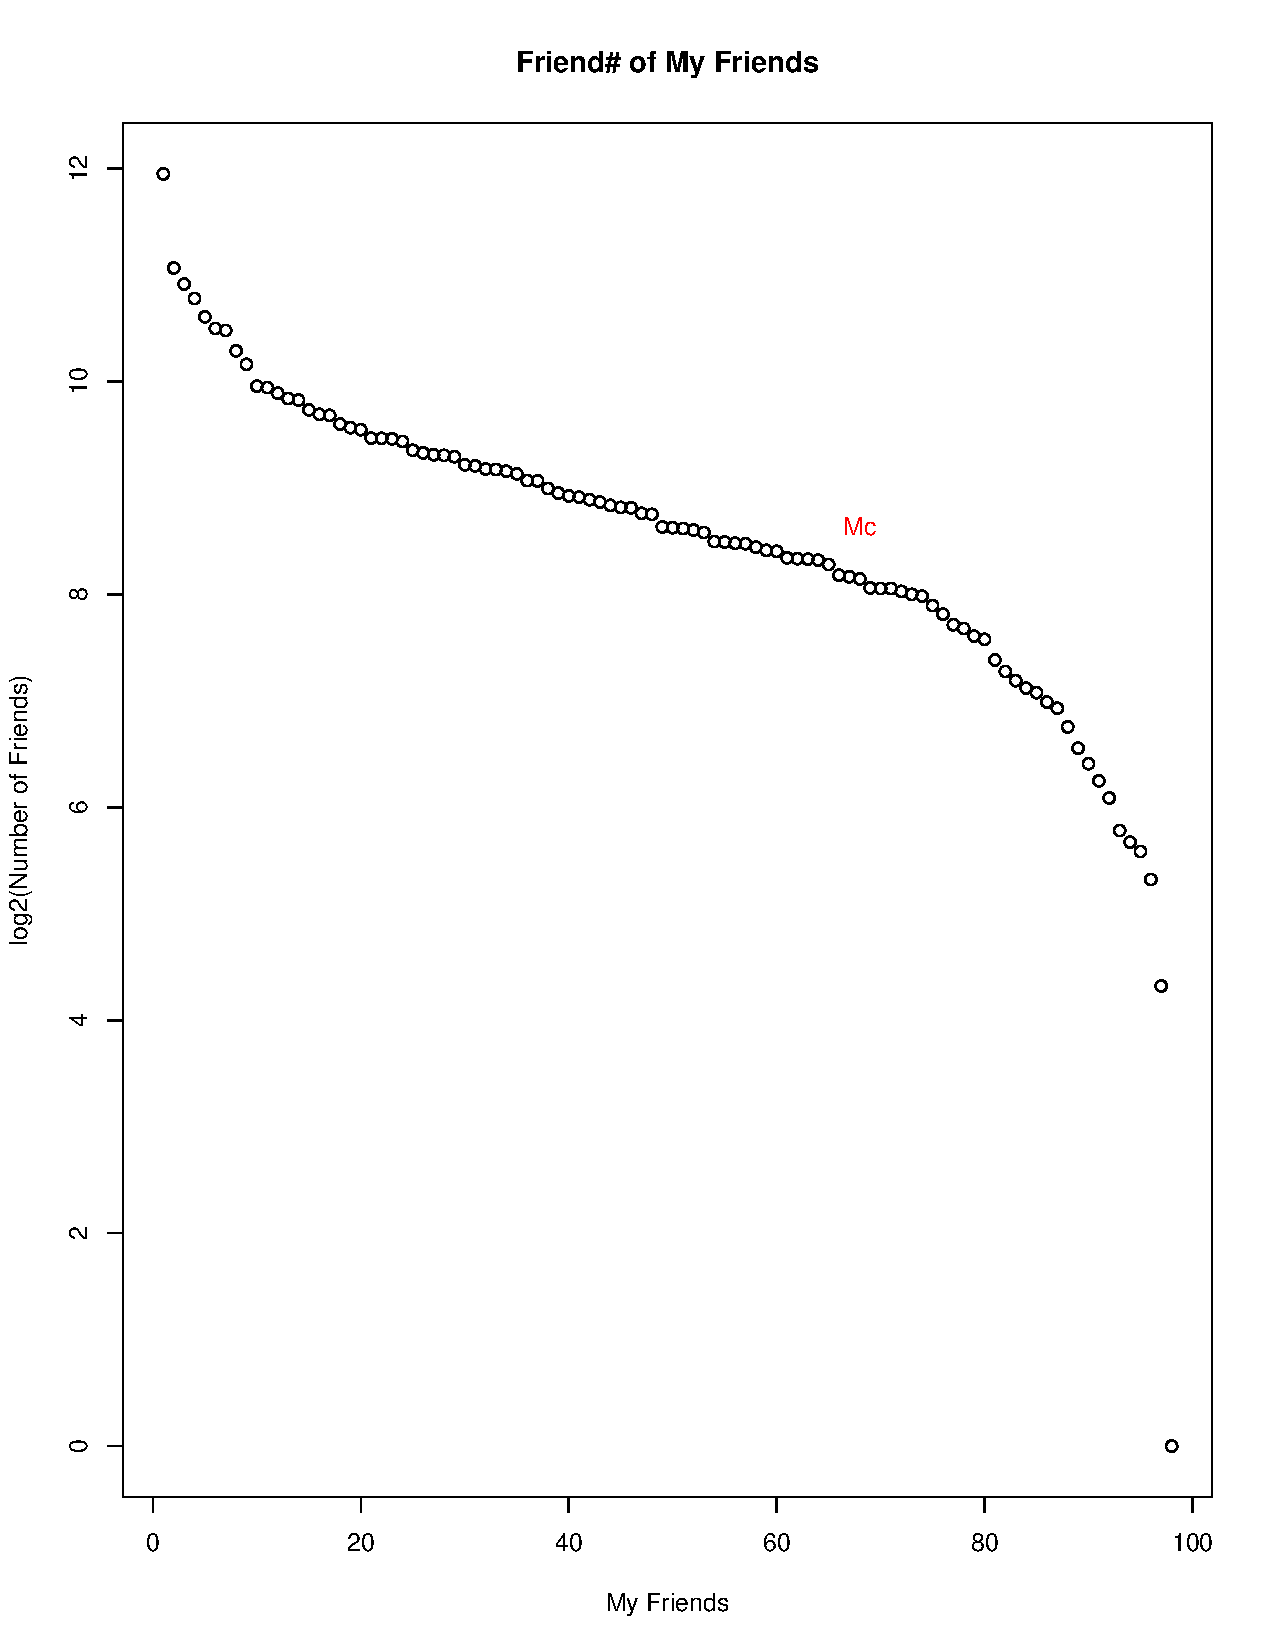
\includegraphics[scale=0.35]{FacebookPlot.pdf}\\
        \caption{Facebook Friendship Paradox Graph}
        \label{Facebook Friendship Paradox Graph}
        \vspace{10mm}

Mean: 538.8247
Median:395
Standard Deviation: 540.8818
\vspace{2mm}

The graph shows that most of Dr. Weigle's friends have more friends than her. Mc represents Dr. Weigle. Both the mean and median are more than her number of friends (283).

\section{Problem 2}

\subsection{Question}
\vspace*{10pt}
Determine if the friendship paradox holds for your Twitter account. Since Twitter is a directed graph, use followers as the value you measure (i.e., "do your followers have more followers than you?").\\

Generate the same graph as in Q1, and calcuate the same mean, standard deviation, and median values.\\

For the Twitter 1.1 API to help gather this data, see:\\

https://developer.twitter.com/en/docs/accounts-and-users/follow-search-get-users/api-reference/get-followers-list

If you have less than 50 followers on Twitter, then you can use my Twitter account (weiglemc).\\

\subsection{Answer}
This approach was similar to the last, except I have to find the Twitter API and use it to get my follower count. I figured out the twitter API limits the number of requests, so I used the follower API to get 200 followers at a time. 
\vspace{1mm}
My Twitter's statistics:
mean: 491.559
median: 228
standard deviation: 25609.87
\vspace{2mm}
\lstinputlisting[language=R, caption={twitterPlotter.r}, label=listing:graphecd]{twitterPlotter.r}
\vspace{2mm}
        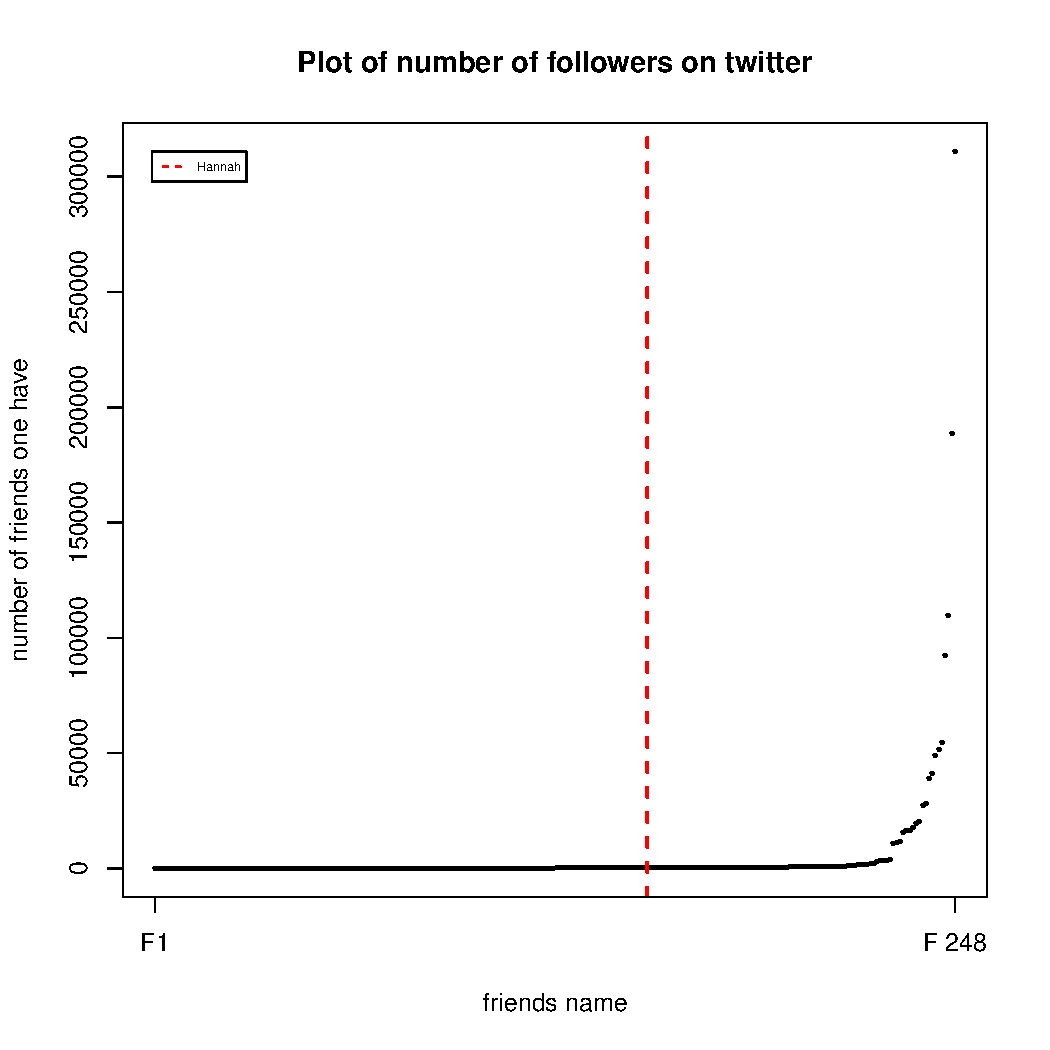
\includegraphics[scale=0.35]{twitterplotter.pdf}\\
        \caption{Twitter Friendship Paradox Graph}
        \label{Twitter Friendship Paradox Graph}
The graph shows many of my followers have more followers than me. So the friendship paradox stands true on this case as well. The mean number of followers is  more than my number of followers (330), but the median isn't (228).

\vspace{2mm}
\vspace*{5pt}

\vspace{2mm}
\vspace{5mm}
\vspace{5mm}

\newpage
\newline
\newpage
\vspace*{5pt}
\bibliographystyle{acm}
\begin{thebibliography}{9}
\bibitem{} Getting Started with Twitter API: \url{http://pr.eyedomain.com/}
\end{thebibliography}
\end{document}
